%********************************************************************
% Appendix B
%*******************************************************
\chapter{Interim Report}
\label{ch:interim_report}
\section*{Introduction} 
\label{sub:introduction} 

%This section should briefly overview the provided topic.
In recent years graphic processing units (GPUs) have moved from fixed pipeline
graphics processors to a fully programmable processor. This evolvment has
attracted many developers to do general purpose computing on GPUs. \glspl{GPU}have
devoted there sillicon (transistors) for computing engines rather than for
control engines like caches, branch prediction, coherency protocols and more.
This incredible computing power made algorithms with an high arithemtic density
run by an order of magnitude faster than on central processing units (CPUs).
Speedups of 100x faster than the CPU were stunning but only a few people
understand why such speedups are possible and why only a couple of algorithm can
attain such speedups.

This thesis will cover all the topics to understand the architecture,
programming model, software eco system, drawback and pittfalls when doing
general purpose computing on GPUs. The \gls{GPU} is a highly parallel processor with
thousands of threads and a peak performance of ~600 GFlops (G92
core\footnote{http://www.nvidia.com/page/geforce\_8800.html}).

Many developers in these days are faced with multicore processors and have to
implement or extend existing algorithms to take full advantage of the
processing power of such cores. CPU manufacturer are facing fundamental problems
when increasing performance only by frequency. In former times higher frequency
meant higher performance but a paradigm shift took place now the new stigma is
more cores means higher performance. Moore's law says that for every 2 years the
amount of cores on a chip will double. What does it mean to developers? They
have to think in parallel, not only for two or four cores but rather for 16 or
32 cores. They have to assure that there code is scaling over many cores over
many generations of CPU chips. There are several parallel programming languages
and middleware to help developers to programm in parallel but a quasi standard
has not been established.

By the means of an application which will be ported to the \gls{GPU} the general
workflow will be shown and various procedure models examined. It will be
presented that often traditional software engineering principles do not
apply to high performance, parallel computing. For this work a Nvidia \gls{GPU} will
be used togehter with \gls{CUDA} (Common Unified Device Architecture) that is a
extension to C for parallel programming of GPUs. 

The remainder of the thesis will give some in depth background to the topic and
expose with programming models and the architecture of GPUs. Furthermore the
development of a parallel implementation of an algorithm will be examined step
by step. In this context software analysis and design principles will be shown
that fit to parallel programming. A feasibility study will cover major obstacles
and show how to avoid them.

Finnaly an application for visualization of complex and chaotic dynamical
systems will be implemented and presented in all aspects to the reader.
% section introduction_ir (end)
\section*{Background to the Project} 
\label{sub:background_to_the_project} 
% This section should provide a more 
% detailed review of the technickal field, largely base upon survey material.
There are many opinions about parallel programming. On the one hand some say
that parallel programming is hard and error prone and on the other hand with the
right tools and programming languages it is a peace of cake. This work will
examine some facts and thoughts about parallel programming and show how one can
identify parallelism, avoid race conditions and tune for performance.
Additionally a modern programming method will be introduced that makes
programming graphics processors easy. The following sections will cover some
major topics which are the basic modules of this thesis. Beginning with the
architecture of modern graphics processors it will be shown how these \glspl{GPU}can
be programmed and at last a simple example implemented in CUDA. 

\subsection*{The Tesla Architecture} % (fold)
\label{sub:the_tesla_architecture}
The Tesla architecture announced 1999 and developed by NVIDIA is the first
GPU highly specialized for raster operations and more important
for general purpose computing. Formerly \glspl{GPU}had fixed-function
pipelines and separate processing units with no ability for programmability to
the vertex and fragment stages of the pipeline. In recent years manufacturers of
GPUs added more and more programmability to the different stages
of the pipeline and at the same time general purpose computing capabilities
\citep{citeulike:3844545}. Furthermore manufacturers introduced the \emph{Unified
Shader Model (USM)} that unifies the processing units allowing for better
utilization of \gls{GPU} resources. The resources needed by different
shaders varies greatly and the unified design can overcome this issue by
balancing the load among vertex, fragment and geometry functionality
\citep{citeulike:3145468}.

\begin{figure}[ht]
\centering
%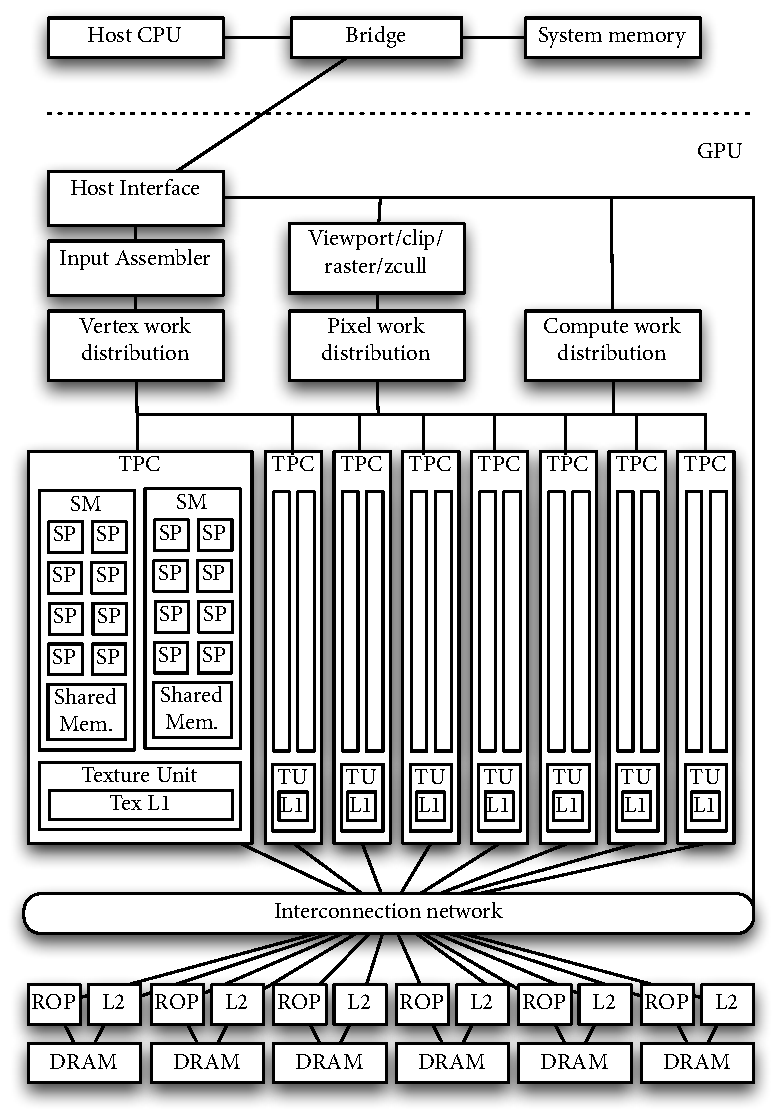
\includegraphics[width=0.6\textwidth]{gfx/tesla_architecture}
\caption{Tesla Architecture}
\label{fig:tesla_architecture}
\end{figure}

The figure \autoref{fig:tesla_architecture} shows the Tesla architectures. As
mentioned above the new \gls{GPU} architectures are a radical departure
from traditional \gls{GPU} design (USM). The Tesla 8 Series has 16 multiprocessors. 
Each multiprocessor is composed of 8 streaming processors, 128 processors in 
total. Each streaming multiprocessor has 16 KB of shared memory
and a L1 cache attached and has access to a texture unit. A streaming processor
consists of a scalar ALU and performs floating point operations. 32 streaming
processor build up a SIMD unit (warp) in that one instruction is executed.
The 8800 GTX has 768 MB of graphics memory, 620 GFlops of peak performance and
86 GB/s peak memory bandwidth. Many massively data-parallel algorithms can be
run sufficiently on this specialized architecture \citep{citeulike:3145468}.
Programming for this architecture is done with \gls{CUDA} (Common Unified Device
Architecture) the C language extension which will be covered in the next
section.
% section the_tesla_architecture (end)


\subsection*{Common Unified Device Architecture (CUDA)} % (fold)
\label{sub:common_unified_device_architecture_cuda_}
In 2007, NVIDIA introduced an extended ANSI C programming model and software
environment the Compute Unified Device Architecture (CUDA). The reason why CUDA
was is born is that parallelism is increasing rapidly with Moore's
law\footnote{Processor count is doubling every 18 - 24 months} and the challenge
is to develop parallel application software that scales transparently with the
number of processor cores. The main goals when \gls{CUDA} was developed were that it
scales to 100s of cores, 1000s of parallel threads and it allows heterogeneous
computing (CPU + GPU). All this considerations led to the result that \gls{CUDA} runs
on any number of processors without recompiling an the parallelism applies to
both \glspl{CPU}and \glspl{GPU}\citep{citeulike:3839013}.

CUDA is C with minimal extensions and defines a programming and memory model.
There are three key abstractions in CUDA, a hierarchy of thread groups, shared
memories and barrier synchronization \citep{citeulike:3325943} that are exposed
to the developer. \gls{CUDA} uses extensive multithreading where threads express
fine-grained instruction, data and thread parallelism that are grouped into
thread blocks which express coarse grained data and task parallelism. The
developer has to rethink about his algorithms to be aggresively parallel.
The problem has to be split into indepedent coarse sub-problems and at finer
level into fine-grained sub-problems that can be solved cooperatively
\citep{citeulike:3325943}.

CUDA has been accepted be many developers which can be seen by the huge amount
of already developed software and contributions to the \gls{CUDA} Zone:
\emph{www.nvidia.com/cuda}. A brief look shows the \gls{CUDA} computing sweet 
spots\citep{citeulike:3839013}: 
\begin{itemize} 
	\item High arithmetic intensity (Dense linera algebra, PDEs, n-body, 
			finite difference, ...) 
	\item High bandwidth (Sequencing (virus scanning, genomics), sorting, 			
			database, ...) 
	\item Visual computing: (Graphics, image processing, tomography, 
			machine vision, ... ) 
	\item Computational modeling, science, engineering, finance, ... 			
\end{itemize}

This is just a small snapshot of algorithms that can be used with \gls{CUDA} on
GPUs. For a more extensive list and speedups compared to high end CPUS see
\emph{www.nvidia.com/cuda} and \emph{www.gpGPU.org}.
 % section common_unified_device_architecture_cuda_ (end)

\subsection*{CUDA Programming Model} % (fold)
\label{sub:cuda_programming_model}
The \gls{CUDA} programming model exposes the graphics processor as a highly
multithreaded coprocessor. The graphics processor is viewed as a compute device
that is a coprocessor to the host that has its own device memory and runs many
threads in parallel.

Applications are accelerated by executing data parallel portions of the
algorithm on the \gls{GPU} as \emph{kernels} which run in parallel on
many threads. There are some major differences between CPU and \gls{GPU} threads. 
A \gls{GPU} needs thousands of threads for full efficience where \glspl{CPU} only need a few of
them. \gls{GPU} threads have a very little creation overhead and are extremely
lightweight compared to CPU threads.

\paragraph{Thread Batching} % (fold)
\label{par:thread_batching}
A kernel is executed as a grid of thread blocks where data memory space is
shared by all threads. A thread block is a batch of threads that can cooperate
with each other by synchronizing there execution\footnote{For hazard free shared
memory access} and efficiently sharing data through the low latency shared
memory. Two threads from two different blocks can cooperate with atomic 
functions through the global memory. The identification of a thread is 
accomplished through block and thread ids which are assigned to each thread at 
creation time. 
% paragraph thread_batching (end)

\paragraph{Block and Thread IDs} % (fold)
\label{par:block_and_thread_ids}
Every thread and block have a unique id. As a result of this each thread can
decide whata data to work on. For every block there is a assigned id in 1D or 2D
layout. Thread ids can be accessed either with 1D, 2D or 3D coordinates similar
to multidimensional arrays. It simplifies memory addresing when processing
multidimensional data. For example image processing, matrix multiplication or
solving partial differential equations on volumes and so on. The data can reside
in several levels of the device memory. 
% paragraph block_and_thread_ids (end)

\paragraph{Device Memory Space} % (fold)
\label{par:device_memory_space}
The memory space is a hierarchy of several memory types that can be accessed per
thread, block, grid and the host. The threads have access to all memory levels
beginning with the read/write (rw) registers, local, shared, global, read only
(ro) texture and constant memory. The grids have only access to global, constant
and texture memory. Whereas the CPU (host) can (rw) global, constant and texture
memories.

Global, constant and texture memory have long latency accesses. They reside off
chip where registers local\footnote{Not true for older \glspl{GPU}chips where local
data is spilled out to global memory} and shared memory reside on-chip. The
global, constant and texture memory are mainly used for communication of (rw)
data between host and device where the contents is visible to all threads. As
mentioned above texture and constant memory can be written by the host where
constants and textures are initialized.
% paragraph device_memory_space (end)


\subsection*{A Simple Example} % (fold)
\label{sub:a_simple_example}
This simple example will show the structure of an \gls{CUDA} program. The executing
kernel will do some easy calculations on the data provided, load the data into
shared memory  and write back the results to the global memory. 

A \gls{CUDA} program has a specific structure where the major parts are described in
this paragraph. The first thing to do is to initialize the device and some
auxiliary variables. Listing \autoref{lst:init} shows the initalization.

%
\begin{lstlisting}[caption=Hardware initalization, label=lst:init]
int main( int argc, char** argv) {
	CUT_DEVICE_INIT(argc, argv);

	uint32_t num_threads = 32;
	uint32_t mem_size = sizeof(float) * num_threads;
	    							
                  ...
\end{lstlisting}
%

Since the \gls{GPU} is attached to the PCIe bus the host has no direct access to 
the global, constant and texture memory and has to transfer the data back
and forth with the DMA engine of the device. This is accomplished through the 
CUDA api calls that initiate the transfer. Before any transfer can be done
one has to allocate memory on the host and on the device for input and output
data. This is shown in listing \autoref{lst:datatransfer}.


\begin{lstlisting}[caption=Data transfer of data, label=lst:datatransfer]
	// allocate host memory 
	float* h_idata = (float*) malloc(mem_size);
	// allocate device memory 
	float* d_idata; cudaMalloc((void**) &d_idata, mem_size);
	// allocate device memory for result
	float* d_odata; cudaMalloc((void**) &d_odata, mem_size);
	// allocate mem for the result on host side
	float* h_odata = (float*) malloc( mem_size);
	// copy host memory to device 
	cudaMemcpy(d_idata, h_idata, mem_size, cudaMemcpyHostToDevice);
\end{lstlisting}


After setting up the input data the setup execution parameters are defined that
are used to startup the kernel. The $grid(1, 1, 1)$ statement defines a
multi-dimensional array of grids $x=1, y=1, z=1$ whereas the
$threads(num\_threads, 1, 1)$ defines a multi-dimensional array of threads
$x=num\_threads, y=1, z=1$ which are actually $1D$ arrays. Listing
\autoref{lst:execution} shows the call of the kernel with its input and output data.


\begin{lstlisting}[caption=Execution of the Kernel, label=lst:execution]
	    // setup execution parameters
	    dim3  grid( 1, 1, 1);
	    dim3  threads(num_threads, 1, 1);

	    // execute the kernel
	    kernel<<< grid, threads, mem_size >>>(d_idata, d_odata);

\end{lstlisting}



If everything went well the host can copy the data from device memory
to host memory and check, visualize or store the calculated values. Listing
\autoref{lst:result} shows the last steps before exiting the program.


\begin{lstlisting}[caption=Retrieving of the Results, label=lst:result]
	    // check if kernel execution generated and error
	    CUT_CHECK_ERROR("Kernel execution failed");
 
	    // copy result from device to host
	    cudaMemcpy(h_odata, d_odata, sizeof( float) * num_threads, 
			       cudaMemcpyDeviceToHost);

	    // cleanup memory free(x), free(y), free(z) ...
		CUT_EXIT(argc, argv);
	}
\end{lstlisting}



The previous listings showed the host code and how to launch a kernel on the
device. The listing \autoref{lst:device} shows the device code portion. There are
several qualifiers that define which function is compiled for which processing
unit. The \textit{\_\_global\_\_} qualifier specifies that this function is run
on the device and hence compiled for the \gls{GPU} where the \textit{\_\_host\_\_}
qualifier specifies that this function is only run on the host and not on the
device. There are more function specifiers that can be looked up in
\citep{citeulike:3325943}.

For data there are as well qualifiers where one can specify where the data is
located, either in constant, global or shared memory. In listing
\autoref{lst:device} the \textit{\_\_shared\_\_} qualifier is used. The device will
use the shared memory to preload the data for faster access.


\begin{lstlisting}[caption=CUDA device code, label=lst:device]
	#include <stdio.h>

	#define SDATA(index) CUT_BANK_CHECKER(sdata, index)
	// Simple test kernel for device functionality
	__global__ void kernel( float* g_idata, float* g_odata) 
	{
	  // shared memory
	  // the size is determined by the host application
	  extern  __shared__  float sdata[];

	  // access thread id
	  const unsigned int tid = threadIdx.x;
	  // access number of threads in this block
	  const unsigned int num_threads = blockDim.x;

	  // read in input data from global memory
	  // use the bank checker macro to check for bank conflicts during host
	  // emulation
	  SDATA(tid) = g_idata[tid];
	  __syncthreads();

	  // perform some computations
	  SDATA(tid) = (float) num_threads * SDATA( tid);
	  __syncthreads();

	  // write data to global memory
	  g_odata[tid] = SDATA(tid);
	}

\end{lstlisting}


After loading the data the kernel just multiplies the thread-id with the number
of threads and saves the result back to global memory where the host can pick up
the result.
% section a_simple_example (end)
% section cuda_programming_model (end)
% section background_to_the_project (end)


\section*{Initial Survey} 
\label{sub:initial_survey} 
% This survey is a quick perliminary survey, to discover something of the shape 
% of the relevant field of information; in doing this you will identify key 
% abstracts, journals, books, series of reports, and so on. Key technical issues 
% will be summarised.
The first thing to answer is why should someone do general purpose computing on
GPUs (GPGPU) anyway. For the most people \glspl{CPU}are just enough. They do not
demand on high computational power and on a high bandwidth. Still there is
paradigm shift taking place and this can not be neglected. As stated in
\citep{citeulike:1187394} and in \citep{citeulike:3421647} CPU manufacturers are
facing problems which they cannnot overcome just by increasing the frequency.
The often cited \emph{Walls} are first, \emph{The Memory
Wall}\citep{citeulike:457955}, \emph{The Frequency Wall} and \emph{The Power
Wall}. The only way seen by CPU makers is currently to go multicore. Intel e.g.
went multicore with there new \emph{Core Microarchitecture} for consumer
products and even a \gls{GPU} replacement, \emph{Larrabee} \citep{citeulike:3153758}.
IBM, Toshiba and Sony developed the \emph{Cell Broadband Architecture} a 9 core
chip \citep{citeulike:1243173}. SUN developed the \emph{Niagara} CPU a multi-core
general purpose processor. It has eight in-order cores, each of them capable of
executing four simultaneous threads \citep{citeulike:3743958}.

Compared to \glspl{CPU}GPUs went years ago to multicore and multithreading. \glspl{GPU}are
maybe the kind of processor where \glspl{CPU}are heading to in terms of multithreading
and raw performance. Forecasts project that every two years the amount of cores
can double. The multicore approach may be the answer to the problems stated
above but this yields to another thing the \emph{parallel programming problem}
\citep{citeulike:3750573}. User will only benefit from this growth if software
can make use of all the cores. Many developers learned about the
single-threaded von neumann model and are not familiar with parallel code which
is subject to errors such as deadlocks and livelock, race conditions and many
more. Parallel programming is difficult and there are several paradigms to make
life easier for developers. 

On of these is the data-parallel paradigm. Where one
is not trying to assign diffferent subtasks to separate cores rather assigning
an individual data element to a separate core for processing
\citep{citeulike:3750565}. 3D rendering, an embarassingly data-parallel problem,
has driven the \gls{GPU} evolution which makes the \gls{GPU} a perfect target for
data-parallel code. There are several fine-grained or data-parallel programming
environments that leverage the \gls{GPU} for general purpose computing (Brook, Sh,
RapidMind, ...). 

The focus of this work will be CUDA\footnote{www.nvidia.com}. \gls{CUDA} is the only
environment which is not based on a graphics library and officialy released by
NVIDIA for their GPUs. \gls{CUDA} is a minimal extension to C and C++ programming
languages. The technique employed by \gls{CUDA} is single process, multiple data
(SPMD). Tasks are split up and run simultaneously on multiple threads (cores)
with different input \citep{citeulike:3072519}.

\subsection*{Choosing a Fast Algorithm} % (fold)
\label{ssub:choosing_a_fast_algorithm}
Before even digging into the wide field of algorithms and difficult problems in
high performance computing one has to understand the hardware architecture of
the \glspl{GPU}to make a decision if an algorithm can be mapped on GPUs. A pretty good
overview over the NVIDIA \gls{GPU} gives the \emph{NVIDIA \gls{CUDA} Programming Guide}
\citep{citeulike:3325943}. A little bit outdatet but still of interest is
\emph{The GeForce 6 Series \gls{GPU} Architecture}\citep{citeulike:3757915} which gives
an overview how the \gls{GPU} fits into the whole system, what a fragment processor,
vertex processor or what textures are. To have a even deeper look into \glspl{GPU}the
article \citep{citeulike:2790995} is highly recommended.

\paragraph{Computations which Map Well to GPUs} % (fold)
\label{par:computations_which_map_well_to_GPUs}
It is important to understand that \glspl{GPU}are good at running computer graphics
and algorithms which \emph{mimic} or have the attributes of computer graphics in
terms of data parallelism and data independence. Not only that similar
computations are applied to streams of many data elements (vertices, fragments,
...) but also the computation of each element is completely or almost completely
independent \citep{citeulike:3733428}. Such types of algorithms are often called
embarassingly parallel algorithms where subtasks rarely or never communicate to
each other.

Another important fact for a algorithm is the \emph{Arithmetic Intensity}. The
Arithmetic Intensity is the ratio of computation to bandwidth or formally:
\begin{center} 
 \emph{arithmetic intensity = operations / words transferred.}
\end{center}
This fact is important because the increase of computational throughput is
faster than the memory throughput which leads to the problem known as \emph{The
Memory Wall}. \gls{GPU} memory systems are architected to deliver high bandwidth,
rather than low-latency, data access. As such computations that benefit most of
the \glspl{GPU}have a high arithmetic intensity \citep{citeulike:3733428}. The next 
sections will represent some algorithms which could fit to GPUs. 
% paragraph computations_which_map_well_to_GPUs (end)

\paragraph{Ray Tracing} % (fold)
\label{par:ray_tracing}
Ray Tracing \citep{citeulike:841961} is an embarrassingly parallel alorithm which
could fit well to GPUs. The author has a extensible knowledge of Ray Tracing on
massively parallel computers \citep{citeulike:80546}. Thats why Ray Tracing was
first considered for porting to the GPU. Unfortuneately there were several
implementations already done for the GPU. Nevertheless equipped with all the
knowledge about Ray Tracing and how to split up the work, arrange the data on a
parallel machine to run efficiently the Ray Tracing algorithm
\citep{citeulike:3770900} will be used for initial benchmarks and the feasibility
study.
% paragraph ray_tracing (end)

\paragraph{Photon Mapping} % (fold)
\label{par:photon_mapping}
Ray Tracing has a local illumination model. To generate more realistic effects
like caustics, diffuse / glossy indirect illumination and more a more
sophisticated model has to be used. Global illumination like \emph{Photon
Mapping} \citep{citeulike:635695} can create all the effects that Ray Tracing
cannot. There are implementations of photon mapping on GPUs
\citep{Purcell:2003:PMO} which are developed with graphics apis and not with
CUDA. Anyhow since photon mapping is heavily using a kd-tree it would be a major
effort to develop an efficient data structure which has the same functionality
as a kd-tree. Nevertheless the first candidate for porting to the \gls{GPU} is \emph{Photon Mapping}.
% paragraph photon_mapping (end)

\paragraph{Multiple Precision Arithmetic} % (fold)
\label{par:multiple_precision_arithmetic}
Another interesting field which demands high computational power is number
theory. The most common/known application is asymmetric cryptography. To
decipher messages that are cyphered with an asymmetric algorithm one needs
superior computational power. An overview over common algorithms gives
\citep{citeulike:3783254}. All algorithms have one thing in common they need a
multiple precision library to represent numbers with 200 and more digits. A good
overview gives \citep{citeulike:3783244}.

The idea was to implement some of the factoring algorithms to the GPU. The only
thing needed is the multiple precision library. In \citep{citeulike:3783254} the
Gnu Multiple Precision (GMP) library was used to implement the algorithms. So
the multiple precision arithmetic is another candidate for porting to the GPU.
% paragraph multiple_precision_arithmetic (end)

\paragraph{High Dynamic Range} % (fold)
\label{par:high_dynamic_range}
Image processing is always a candidate for embarassingly parallel algorithms. A
pretty new algorithm to enhance images is \emph{tone mapping}
\citep{citeulike:3783303}. Tone mapping is the compression of dynamics in High
Dynamic Range (HDR) pictures. There are several algorithms for tone mapping:
Mantiuk \citep{citeulike:3783315}, Reinhard \citep{citeulike:3783311}, Durand
\citep{citeulike:789299}, Fattal \citep{citeulike:3783313} and many more. All of
this algorithms are present in the pfs-tools library written by Krawczyk
\citep{citeulike:3783303}. As this document was written Krawczyk was already
implementing the pfs-tools on \gls{GPU} but not publishing it. Furthermore there is an
complete editor written for hdr image processing which is running on the GPU. So
HDR was discarded but there are several other algorithms in image processing
which are considered as candidates. Some algorithms in no particular order:
segmentation, tracking, filtering, ... and so on. This is put as another
candidate to the list of the possible algorithms for porting. 
%paragraphhigh_dynamic_range (end)

\paragraph{Genetic Algorithms} % (fold)
\label{par:genetic_algorithms}
Parallel genetic algorithms are usually implemented on parallel machines but
fine-grained parallel genetic algorithms can be mapped to GPUs
\citep{citeulike:3801879}. In \citep{citeulike:3801866} its shown what kind of
genetic algorithm map well to \glspl{GPU}and how the work and communication is
handled. It is \emph{pretty} easy to implement simple genetic algorithms on the
GPUs but with increasing complexity one has to consider many more things: load
balancing, communication pattern, dynamic memory allocation, resolving of
recursion ... . Another paper \citep{citeulike:3801883} compares genetic
algorithms implemented on \glspl{CPU}and \glspl{GPU}and shows that the latter is much more
effective than the former. All genetic algorithms have one thing in common the
core algorithm. Once effectively implemented on the \gls{GPU} the core algorithm is
extended with definitions like the population, selection, recombination and
mutation to solve a specific problem. The skill here is to choose the right
definitions and not more the efficient implementation of the core algorithm. So
this topic excluded from the candidate list.
% paragraph genetic_algorithms (end)

\paragraph{Chaos Theory} % (fold)
\label{par:chaos_theory}
Another interesting field is chaos theory. Especially the visualization of
chaos. The maybe most famous visualization of chaos is \emph{The Fractal Flames
Algorithm}. Fractal flames are a member of iterated function system class of
fractals created by Scott Draves \citep{citeulike:3801950}. He uses a rather
complicated set of functions in the system to generate stunning visualization of
the iterative process of the system. The next release will have support for the
GPU. Thats why it was firstly discarded but the research about chaos led to
other interesting papers respectively books.

There is no need to use approx. 21 function for a system to generate visually
appealing pictures of chaos. Sprott showed in \citep{citeulike:3745535} that even
with very simple functions one can create patterns in chaos. This patterns are
called \emph{Strange Attractors} and are the visualization of chaotic behaviour.
There are created by iterating a simple equation some million times. 

Pickover shows in his book \citep{citeulike:3812233} how to create patterns from
a variety of sources. He shows how to create nice looking patterns from fourier
analysis, acoustic, chemistry and many more. Anyhow all of these equations or
differential systems have on thing in common no matter how complicated the
system is the core algorithm is to iterate a specific equation with correct
input numbers to create chaos. The algorithm is heavily computational bound
which makes it a good candidate for porting to the GPU.
% paragraph chaos_theory (end)
% section choosing_a_fast_algorithm (end)
\subsection*{Summary} % (fold)
\label{ssub:summary}
After examining many possible candidates which can be accelerated with an GPU,
some of them were already in progress, some other maybe not feasible in the
timeframe of a master thesis. Nevertheless one algorithm has to be chosen and
this specific one will be ported to the GPU.

By the means of this example the typical data parallel programming approach will
be shown and it will be illustrated how to think in paralllel.
% section summary (end)
% section initial_survey (end)
\section*{Aims and Objectives} 
\label{sub:aims_and_objectives} 
% A clear statement of the Aims and Objectives. Remember, aims and objectives 
% are generally a statement of what is to be achieved, not how it is to be
% achieved.

% The aim gives you a general indication of what you might learn and how you
% might benefit from a course. However, it does not give you any details, or a
% means of assessing whether your learning has been successful. Objectives are
% used for this purpose.

One aim of this master thesis is to show whether graphic cards are suitable for 
general purpose computing. With an algorithm example that is running slow on a 
CPU the process of porting to a \gls{GPU} is examined. As a result, the algorithm
will be running by a magnitude faster on the GPU. 

Another aim is to understand the architecture and programming models of GPUs.
Therefore the algorithmic view to \glspl{GPU}will be presented and computational
concepts and efficient data structures explained. Understanding these key
concepts makes one understand the architecture of GPUs.

% The objectives tell you what you should be able to do after the course, eg on
% completion of this programme the learner will: 

% - be able to identify key principles of adult teaching and learning 
% - be able to apply educational techniques learned to everyday teaching and 
% supervision 
% have identified their own strengths and weaknesses in teaching and
% supervision. The objectives 
Dissasociation from sequential algorithms and thinking in parallel will be one
major discipline after working through this thesis. On will be able identify
algorithms that are well suited for \glspl{GPU}and design efficient data flow and high
performing code.

Assessment of algorithms, knowledge about \gls{GPU} architecture, program flow and
data access patterns make one able to rate if a \gls{GPU} is suitable for general
purpose computing.
% section aims_and_objectives (end)

\section*{Experimental/Investigative methods to be adopted} 
\label{ssub:experimental_investigative_methods_to_be_adopted} 
% An outline of the key activities necessary to complete the project, itemising
% the experimental methods to tebe used (in, for example, a design-based 
% project), or the investigative techniques to be adopted (in the case of, say, 
% a critical survey).
To estimate if an algorithm is suitable for running on the \gls{GPU} first of all the
hardware architecture has to be understood. Since \glspl{GPU}are \emph{completely}
different than \glspl{CPU}one has to understand how simple things like loops,
arithmetic, data access and program flow are managed on such hardware. The most
interesting part here is the fact that \glspl{GPU}are able to hold up to approx. 12000
threads in flight. Understanding the hardware is the key for high performance 
computing on GPUs.

To get an impression how one can/should write code for \glspl{GPU}a feasibility study
will be done that will show answers to statements stated above and further 
questions. 

Further questions arise when reading scientific papers about general purpose
computing on graphics hardware. Often there are statements which are not
applicable to current hardware generation. These limitation arise from the fact
that the \glspl{GPU}are implementing a graphics pipeline that is \emph{normally} used
for rasterization and rendering. The developers where confronted with an
graphics API and a graphics pipeline which thinks of triangles and pixel rather
than floats and integers. As a result the developers had to think about how to
rotate, scale or translate a triangle to perform a calculation in an algorithm.
There are several myths and truths about general purpose computing on graphics 
hardware which will be answered with the evolvment of the feasibility study. 

Since general purpose computing on graphics hardware is not more or less 'C'
programming with some extension, the best way to learn programming for \glspl{GPU}ist
learning by doing. Therefore several algorithms (Box Filter, Gaussian Blur, HDR,
... ) and further more will be studied.
This way one will get enough experience to structure a initial code and have
clue about how to split the work apart, offload computational intensive parts to
the \gls{GPU} and let do the general purpose processor the io and input handling.

Simple micro, synthetic\footnote{Synthetic benchmarks mimic a particular type of
workload on a component or system. Whereas application benchmarks run real world
programs} benchmarks are often used to describe the hardware by their peak
numbers. Either gflops achieveable or the bandwith between the processing unit
and the memory. They can easily show the basic conditions which one has to face 
with. Several benchmarks are already available in the SDK so only a few have to 
be developed. One critical point in general purpose computing is called
arithmetic density. Which describes how many arithmetic operations are executed
before another load is needed to fetch data. Micro benchmarks can easily show 
how arithmetic density effects performance, which in conclusion can show how 
performant an application will run on the GPU. 

The steps above will lead to a pretty good understanding of the hardware which
leads to the next step the searching and identifying a suitable algorithm to
port to the GPU. A critical survey of algorithms that are ported to \glspl{GPU}and
that are not ported will be done. There are many high performance algorithms out
there which take \emph{forever} to complete. If its chemistry, physics, biology,
astronomie and mathematics all of them can be ported to a \gls{GPU} to some extent. It
is important to fetch the applicable one and by means of that algorithm to show
the analysis and design process of high performance programs. There are
several things to consider when designing for parallel hardware which will be
examined an explained in the responsible chapters.

% section experimental_investigative_methods_to_be_adopted (end)
\section*{Time-plan} 
\label{sub:time_plan} 
%Strongly related to the key activities identified above.
For the project \emph{General Purpose Computing on Graphics Hardware} the
following milestones were defined and listed below. Each milestone will have a
short description which tasks have to be accomplished to complete a mile stone.
With every milestone a chapter respectively a section of the master thesis will
be written which corresponds to the current carried out milestone. So the 
development of the milestones goes hand in hand with editing of the thesis.

\paragraph{M0: Interim Report (1/31/2009)} % (fold)
\label{par:interim_report}
For this milestone following tasks were done, the conduct of the initial survey 
and the writing of the interim report. The initial survey will give a coarse 
overview over the field and related work. 
% paragraph interim_report (end)

\paragraph{M1: Related Work Identified (2/14/2009)} % (fold)
\label{par:m1_related_work_identified}
The next step to take is to identify related work, conducting the literature 
survey. This survey should show the demand of GPGPU and used algorithms. 
Furhtermore it will help to understand the architecture and programming models. 
After gaining enough knowledge about the field its time to get the hands on the 
GPU.
% paragraph m1_related_work_identified (end)
\paragraph{M2: Algorithmic view understood (2/28/2009)} % (fold)
\label{par:m2_architecture_algorithmic_view_understood}
Equipped with the knowledge from the latter milestone it is time to understand
how the architecture works by examining algorithms already mapped to the GPU.
This step is crucial as it shows how algorithms map to and work on the \gls{GPU}
and a good understanding of the environment can help later on for choosing the
right algorithm for porting, analysis, design and implementation.
% paragraph m2_architecture_algorithmic_view_understood (end)
\paragraph{M3: Feasibility Study (3/14/2009)} % (fold)
\label{par:m3_feasibility_study}
The feasiblity study will be used for the first steps into GPGPU. A low featured
ray tracer will be used for examining what the hurdles and obstacles are when 
developing for the GPU. The knowledge will be used for choosing the right 
algorithm. 
% paragraph m3_feasibility_study (end)
\paragraph{M4: Application, Algorithm choosen (3/21/2009)} % (fold)
\label{par:m4_application_algorithm_choosen}
After completion of this milestone the algorithm is chosen to be ported to the 
GPU. So the next milestones will be concentrated only on this algorithm and not 
more generaly. 
% paragraph m4_application_algorithm_choosen (end)
\paragraph{M5: Analysis, Solution Proposed (4/4/2009)} % (fold)
\label{par:m5_analysis_solution_proposed}
Here a solution will be proposed and outstanding issues will be identified. 
There are several myths about GPGPU which will be stated here as well, because 
there are affecting the design of the application and cannot be discarded.
% paragraph m5_analysis_solution_proposed (end)
\paragraph{M6: Experiments (4/14/2009)} % (fold)
\label{par:m6_experiments}
To exclude all eventualities a set of experiments will be undertaken. This will 
as well solve all myths.
% paragraph m6_experiments (end)
\paragraph{M7: Design, Application Ported (5/14/2009)} % (fold)
\label{par:m7_design_application_ported}
This milestone will cover the design of the application with all constraints,
obstacles and hurdles that are involved with GPGPU. In this task the application
will be implemented and run on the GPU. A good implementation will need several
iterations were several aspects will be tuned: coalesced memory access, load
balancing and many more.
% paragraph m7_design_application_ported (end)
\paragraph{M8: Discussion (5/22/2009)} % (fold)
\label{par:m8_discussion}
Another important part is the discussion of the results and methodologies
applied which will be done in this milestone.
% paragraph m8_discussion (end)

\paragraph{M9: Master Thesis Edited (5/30/2009)} % (fold)
\label{par:master_thesis_edited}
Here the thesis will be recaped and briefly outlined. Conclusions will be drawn
and future work presented. A critical summary and conclusion will be provided as
well. % paragraph master_thesis_edited (end)

% section time_plan (end)
\section*{Deliverables or specific outcomes} 
\label{sub:deliverables_or_specific_outcomes} 
% A clear statement of the expected outcome(s).
The main outcome of this work is to show how \glspl{GPU}can be utilized for general
purpose computing. There is a high demand on performance and computational power
for scientific algorithms. Developers search for new architectures to solve
problems in shorter time. One promising new architecture or hardware is the GPU.
Since years \glspl{GPU}were only used for rendering. The switch from fixed pipelines
to programmable pipelines let developers think about using \glspl{GPU}for general
purpose computing. Accidently thery were forced to use 3D apis
(OpenGL\footnote{http://www.opengl.org},
DirectX\footnote{http://www.microsoft.com}) to accomplish task like matrix
multiplication or fast fourier transformation. Nowadays developer use \gls{CUDA}or
middleware like RapidMind to develop software for (NVIDIA) GPUs. It will be
shown that \gls{CUDA}is highly efficient and easy to program which makes general
purpose computing more feasible.

By the means of a application that is computationally intensive it will be shown
that traditional software engineering principles often do not apply to high
performance, parallel computing. Data access is the biggest problem of an
alogirthm to attain maximum performance. If the algorithm is memory bound and
not computational bound the limiting factor or bottleneck is the bandwidth to
the memory. Good data design is essential for good (performant) code. The data
and how it is used must be known in order to effectively design and optimize a
application for a \gls{GPU} or other highly parallel systems like the Cell processor
(Meine Diplomarbiet link). A simple computationally bound algorithm can be
easily designed in a way that it becomes memory bound if data arrangemnet and
access is neglected by the developer. The outcome of all the considerations will
be another approach how to tackle software design on such massively parallel
architecture.

Furthermore a workflow will be presented that shows how to port sequential code
to a massively parallel architecture. Software developer often only need to
compile their code with another compiler to \emph{port} the code to another
architecture. x86 -> PowerPC, x86 -> MIPS ... but the situation for parallel
processors like the cell, niagara and here the \gls{GPU} is completely different. One
has to identify the critical parts and explicitly offload tasks to the GPU. It
is obviuos that this is not the only step to do. Furthermore there are other
facts which have to be considered, like load-balancing, deadlocks, concurrency,
cache coherency and other. A workflow which can be adapted to different parallel
machines is another outcome of this work.

Last but not least is the outlook on future hardware development and programming
models. The problem with new hardware architectures is they have to be accepted
by the developers to succeed in industry. One way to achieve this is to have an
easy programming model which adapts easily to common apis and existing systems.
There are rarely branches of industry which want to, or are able to rewrite
their code for bleeding edge architectures like the cell or \glspl{GPU}if the outcome
is only 2x faster code. In this case many just extend their cluster with another
bunch of \emph{cheap} systems. A factor of 10 is an undocumented limit when to
invest in other, faster hardware.
% section deliverables_or_specific_outcomes (end)

